\input{header}
\AtBeginSection[]
{
	\begin{frame}<beamer>
		\frametitle{Outline}
		\tableofcontents[current,currentsubsection]
	\end{frame}
}

\begin{document}

\begin{frame}[allowframebreaks] \frametitle{Mathematical notions}
  \begin{itemize}

\item Set

Omitted
\item Sequence and tuples

  \begin{itemize}
  \item Sequence: Objects in order
    \begin{equation*}
      (7,21,57) \neq (57,7,21)
    \end{equation*}
  \item Repetition
    \begin{eqnarray*}
      && \mbox{set}: \{7,21,57\}=\{7,7,21,57\}\\
&& \mbox{sequences}: (7,21,57) \neq (7,7,21,57)
    \end{eqnarray*}
  \item Tuples: finite sequence

(7,21,57): 3-tuple
  \end{itemize}
  \item Cartesian product:
    \begin{eqnarray*}
      && A =\{1,2\}, B=\{x,y\}\\
 && A \times B = \{ (1,x), (1,y), (2,x), (2,y)\}
    \end{eqnarray*}
  \item Function: single output
  \item Relation: scissors-paper-stone
    \begin{center}
    \begin{tabular}{lccc}
      beats & scissors & paper & stone \\
scissors & F & T & F \\
paper & F & F & T\\
stone & T & F & F
    \end{tabular}
  \end{center}
  \item Equivalence relation
    \begin{enumerate}
    \item reflexive
      \begin{equation*}
        \forall x, xRx
      \end{equation*}
    \item symmetric 
      \begin{equation*}
        xRy \Leftrightarrow yRx
      \end{equation*}
    \item transitive
      \begin{equation*}
        xRy, yRz \Rightarrow xRz
      \end{equation*}
    \end{enumerate}
  e.g. ``=''
\item Example: $i \equiv_7 j$ if $0 =i -j\mod 7$
  \begin{eqnarray*}
&& i - i \mod 7 = 0\\
&& i - j = 7a, j-i=-7a\\
&& i-j = 7a, j-k = 7b\\
&& \Rightarrow i-k = 7(a+b)   
  \end{eqnarray*}

\item Graph

\item [] Undirected

  \begin{center}
    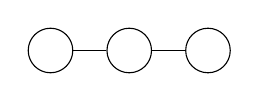
\begin{tikzpicture}
[inner sep=2mm]      
\path ( 0,0) node (1) [shape=circle,draw] {}
( 1,0) node (2) [shape=circle,draw] {}
( 2,0) node (3) [shape=circle,draw] {};
\draw [-] (1) -- (2);
\draw [-] (2) -- (3);
\end{tikzpicture}
\end{center}


\item [] Directed

  \begin{center}
    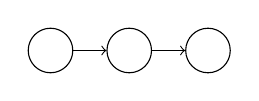
\begin{tikzpicture}
[inner sep=2mm]      
\path ( 0,0) node (1) [shape=circle,draw] {}
( 1,0) node (2) [shape=circle,draw] {}
( 2,0) node (3) [shape=circle,draw] {};
\draw [->] (1) -- (2);
\draw [->] (2) -- (3);
\end{tikzpicture}
\end{center}

\item [] Nodes (vertices)

\item Edges: connection between nodes

\item [] Degree = \# edges at a node

\item [] Subgraph: $G$ is subgraph of $H$ if 

\begin{itemize}
\item $G$ is a graph
\item node($G$) $\subset$ node(H)
\item edge($G$) = subset of edge(H) connecting node(G)
\end{itemize}
\item [] In our example,
  \begin{center}
    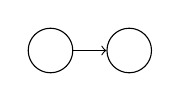
\begin{tikzpicture}
[inner sep=2mm]      
\path ( 0,0) node (1) [shape=circle,draw] {}
( 1,0) node (2) [shape=circle,draw] {};
\draw [->] (1) -- (2);
\end{tikzpicture}
\end{center}
is a subgraph, but
  \begin{center}
    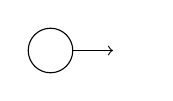
\begin{tikzpicture}
[inner sep=2mm]      
\path ( 0,0) node (1) [shape=circle,draw] {}
( 1,0) node (2) {};
\draw [->] (1) -- (2);
\end{tikzpicture}
\end{center}
is not
\item Strings and languages
  \begin{itemize}
  \item alphabet: $\{0,1\}$
  \item string: 1001
  \item language: set of strings
  \end{itemize}
\item Boolean logic
  \begin{itemize}
  \item true and false
  \item 0 (false) and 1 (true)
  \item $0 \wedge 0 = 0, 0 \vee 0 = 0, \neg 0=1$ (negation operation)
  \item xor $\otimes$
    \begin{gather*}
      0 \otimes 0 = 0\\
0\otimes 1 = 1\\
1 \otimes 0 = 1\\
1\otimes 1 = 0
    \end{gather*}
  \item implication

    \begin{center}
      \begin{tabular}{ll|c}
        $P$ & $Q$ & $P \rightarrow Q$ \\ \hline
        0& 0 & 1\\ 
        0& 1 & 1\\
        1& 0 & 0\\
        1& 1 & 1
      \end{tabular}
    \end{center}
  \item [] Why
    \begin{equation*}
      P = 0, Q = 1, \text{ then } P \rightarrow Q = 1
    \end{equation*}
Consider
\begin{center}
rainy $\rightarrow$ wet land
\end{center}
If not rainy, 
saying rainy implies wet land is ok.
\item $P \rightarrow Q \equiv 
\neg P \vee Q$
    \begin{center}
      \begin{tabular}{ll|c|cc}
        $P$ & $Q$ & $P \rightarrow Q$ & $\neg P$ & $\neg P \vee Q$\\ \hline
        0& 0 & 1 & 1 & 1\\ 
        0& 1 & 1 & 1 & 1\\
        1& 0 & 0 & 0 & 0\\
        1& 1 & 1 & 0 & 1
      \end{tabular}
    \end{center}
  \end{itemize}

\end{itemize}\end{frame} \begin{frame}[allowframebreaks] \frametitle{Proof}
  \begin{itemize}  
  \item Direct proof:
    $$A\rightarrow B$$
  \item Proof by contradiction
    $$\neg B \rightarrow \neg A$$

    \begin{center}
      \begin{tabular}{ll|c|llc}
        $P$ & $Q$ & $P \rightarrow Q$ & $\neg Q$ & $\neg P$ & $\neg Q \rightarrow \neg P$\\ \hline
        0& 0 & 1 & 1 & 1 & 1\\ 
        0& 1 & 1 & 0 & 1 & 1\\
        1& 0 & 0 & 1 & 0 & 0\\
        1& 1 & 1 & 0 & 0 & 1
      \end{tabular}
    \end{center}
    
  \item Example 1:

Every graph $\Rightarrow$ sum of degrees is even
\begin{itemize}
\item An example:
    \begin{center}
    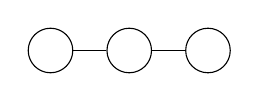
\begin{tikzpicture}
[inner sep=2mm]      
\path ( 0,0) node (1) [shape=circle,draw] {}
( 1,0) node (2) [shape=circle,draw] {}
( 2,0) node (3) [shape=circle,draw] {};
\draw [-] (1) -- (2);
\draw [-] (2) -- (3);
\end{tikzpicture}
\end{center}
\# degrees = 1 + 2 + 1 = 4
\item Each edge: 2 nodes
  \begin{center}
total \# degrees = $2\times $ \# edges
\end{center}
\end{itemize}

\item Example 2: $\sqrt{2}$ is irrational
  \begin{itemize}
  \item The implication
    \begin{equation*}
      \begin{split}
&   \text{Definition of rational numbers}\\
\Rightarrow&  \sqrt{2} \text{ is not rational}
\end{split}
\end{equation*}
That is,
    \begin{equation*}
      \begin{split}
&   \text{If a rational number is ...}\\
\Rightarrow&  \sqrt{2} \text{ is not rational}
\end{split}
\end{equation*}
The opposite is
    \begin{equation*}
      \begin{split}
        &  \text{If $\sqrt{2}$ is rational}
\\
\Rightarrow& \text{The rational number cannot be defined as ...}\\
\end{split}
\end{equation*}
  \item If $\sqrt{2}$ is rational
    \begin{equation*}
      \sqrt{2}=\frac{m}{n}
    \end{equation*}
    and
    $m,n$ have no common factor
  \item Then
    \begin{equation*}
      2n^2=m^2
    \end{equation*}
Looks impossible. But how to write this formally?
\item First we prove that $m$ must be even. This is also proof by
  contradiction
\item [] If $m$ is not even, 
  \begin{equation*}
    m = 2k + 1.
  \end{equation*}
Then
\begin{equation*}
  m^2 = 4(k^2 + k) + 1
\end{equation*}
is not even and
\begin{equation*}
  m^2 = 2n^2
\end{equation*}
does not hold.
\item Now suppose $m$ is even
  $$m=2k$$
\item [] Then
  \begin{equation*}
    n^2 = 2k^2
  \end{equation*}
\item By the same argument, $n$ is even
\item Thus $m, n$ have a common factor $2$ and there
is a contradiction
  \end{itemize}

\end{itemize}\end{frame}


\end{document}
